\documentclass[journal]{IEEEtran}

\usepackage{amsmath}
\usepackage{amssymb}
\usepackage{amsfonts}
\usepackage{graphicx}
\usepackage{textcomp}
\usepackage{booktabs}
\usepackage{listings}
\usepackage[hidelinks]{hyperref}

\lstset{basicstyle=\footnotesize\ttfamily,frame=single,
        breaklines=true,columns=fullflexible,keepspaces=true,
        showstringspaces=false,captionpos=b,abovecaptionskip=2pt}

\begin{document}

\title{Non-Stationarity of Long-Term Memory in Financial Volatility\\
and Its Predictive Value: Empirical Evidence and Implications\\
for Memory-Adaptive Attention in Transformers}

\author{Daria~D.~Bondarenko%
\thanks{Department of Probability Theory and Mathematical Statistics, Belarusian State
University, Minsk, Republic of Belarus (e-mail: adarka.bon@gmail.com).}}

\maketitle

\begin{abstract}
Volatility forecasting is a core problem of modern financial analysis, and the accuracy of
volatility models directly determines the quality of market-risk measures, capital allocation
and derivative pricing. Financial volatility is known to exhibit long-term memory, i.e.\ the slow,
power-law decay of the autocorrelation function, and this effect underlies the FIGARCH,
ARFIMA-RV and HAR-RV model families. A growing body of evidence indicates, however, that the
\emph{strength} of this memory is not a constant characteristic of the process but a dynamic,
regime-dependent property that weakens in crisis periods. Existing deep-learning architectures do
not exploit this fact. The self-attention mechanism of the Transformer behaves as a learnable
autocorrelation function, yet the attention schemes of Informer, Autoformer, FEDformer and
PatchTST are specified a priori and therefore do not follow the current memory regime. Using daily
data for ten assets (five equities, two cryptocurrencies and three currency pairs) over
2019--2023, we estimate the local memory of realised volatility by rescaled-range analysis and by
the Geweke--Porter-Hudak estimator in a rolling window of 500 observations, and test for
structural breaks in the resulting trajectories with a CUSUM test. The local memory parameter
$\hat d$ of realised volatility is found to be significantly non-stationary for seven of the ten
assets and to collapse during crises, the mean value falling from $0.52$ to $0.45$. Adding the
local memory estimate and its first difference to HAR-RV improves the mean-squared error for all
ten assets (on average by $+7.1\%$) and the QLIKE loss for eight of ten (on average by
$+1.8\%$). A pilot experiment on minute-frequency quotes shows that the static attention
mechanisms Standard, ProbSparse and MultiFeature degrade by $+51\%$, $+143\%$ and $+50\%$ in
RMSE respectively when the memory regime switches. On this basis we formulate the
Memory-Adaptive Attention mechanism, in which a differentiable local memory estimator acts as a
control signal adapting the context length and the sparsity of attention to the current memory
regime, and we outline the corresponding VaR/ES backtesting programme. We also discuss in detail
the recent critique of long-memory diagnostics, and argue that the quantity studied here is
better characterised as a time-varying diagnostic of persistence than as an estimate of a
structural fractional integration parameter.
\end{abstract}

\begin{IEEEkeywords}
Long-term memory, realised volatility, non-stationarity, Hurst exponent, Geweke--Porter-Hudak
estimator, HAR-RV, Transformer, self-attention, volatility forecasting, Value-at-Risk.
\end{IEEEkeywords}

\section{Introduction}
\label{sec:intro}

\subsection{Motivation}

Volatility, a measure of the intensity of price fluctuations of a financial asset, is a central
object of study in financial economics and a key input of risk management practice. The accuracy of
volatility forecasts determines the precision of risk measures such as Value-at-Risk and Expected
Shortfall, the capital that must be held against market risk, the pricing of derivative
instruments and the construction of efficient portfolios. The modelling of volatility has followed a
clearly traceable path over the last three decades: from conditional heteroskedasticity models of
the GARCH family and their fractionally integrated generalisations, through realised volatility
models such as HAR-RV, to deep-learning architectures in which the attention mechanism replaces an
explicit multi-scale autoregressive structure.

Two features of volatility have shaped this development, and the second has received markedly less
attention than the first. The first is \emph{long memory}: the autocorrelation function of
volatility decays hyperbolically rather than exponentially, so that observations hundreds of steps
away retain a statistically significant influence on current dynamics. The second, and far less
exploited, is that the \emph{strength} of this memory changes over time. Empirical studies report
that the persistence of volatility is systematically lower in turbulent periods than in calm ones
\cite{ding1993long,andersen2003modeling,vogl2023hurst}. A model that treats the memory structure
as fixed is therefore mis-specified precisely in the periods in which the consequences of
mis-specification are most costly, and the resulting errors are systematic rather than random.

\subsection{The research problem}

The problem addressed in this paper is stated in the language of research design. A research
problem is a specific issue, difficulty or gap in knowledge that one aims to address; it is
distinct from the purpose, i.e.\ from the plan by which one intends to address it
\cite{cherenda2020research}. The problem here is formulated as follows.

\emph{Research problem.} The strength of long-term memory in the volatility of financial time
series is a non-stationary, regime-dependent property. Models that impose a fixed memory
structure --- both the classical econometric families and the current Transformer-based
forecasters --- are therefore systematically mis-specified at regime changes, and a mechanism
that adapts to the locally estimated memory is required.

This statement has three components which we separate deliberately. The first is empirical: is the
memory genuinely non-stationary, and is the change attributable to identifiable regimes? The
second is informational: does the \emph{local} estimate of the memory parameter carry predictive
content that is not already contained in the standard HAR-RV specification? The third is
architectural: do existing static attention mechanisms degrade differently across memory regimes,
which would motivate an adaptive alternative?

\subsection{Research questions and contributions}

Three questions are addressed.

\begin{enumerate}
\item \textbf{Q1.} Is long-term memory in financial volatility genuinely non-stationary, and can
the change be tied to identifiable market regimes?
\item \textbf{Q2.} Does the local estimate of the memory parameter carry predictive information
about future volatility that is not already contained in the standard HAR-RV specification?
\item \textbf{Q3.} Do existing static attention mechanisms degrade differently across memory
regimes, and is any of them uniformly optimal?
\end{enumerate}

The contribution of the paper is fourfold. First, it provides a systematic empirical
demonstration that long-term memory in realised volatility is non-stationary across a
heterogeneous cross-section of ten assets from three asset classes, and that the weakening of the
memory is regime-linked rather than asset-specific. Second, it establishes that the local memory
estimate carries independent forecasting content, quantified through a controlled out-of-sample
comparison against the HAR-RV benchmark. Third, it translates the statistical evidence into a
machine-learning design principle: since self-attention constitutes a learnable autocorrelation
function, an attention scheme that is fixed a priori cannot be optimal across regimes, and the
quantitative degradation reported here demonstrates the size of the effect that an adaptive
mechanism would have to capture. Fourth, and importantly for the interpretation of the results,
the paper engages explicitly with the recent critique of long-memory diagnostics
\cite{gatheral2018rough} and delineates precisely what our estimates do and do not measure.

\subsection{Organisation of the paper}

Section~\ref{sec:related} develops the theoretical background and reviews the literature.
Section~\ref{sec:data} describes the data and the software implementation. Section
\ref{sec:method} presents the estimation of the local memory parameter, the testing procedure for
non-stationarity, the forecasting experiment, the attention experiment, and the formulation of
the Memory-Adaptive Attention mechanism. Section~\ref{sec:results} reports the results.
Section~\ref{sec:discussion} interprets them and states the limitations. Section~\ref{sec:concl}
concludes and sets out the research programme, which follows the programme set out in
Section~\ref{sec:intro}.

\section{Background and related work}\label{sec:related}

\subsection{Long-range dependence: definition and spectral characterisation}

Long-range dependence (LRD) is a property of a stationary process in which the statistical
dependence between observations decays as a power law rather than exponentially, in the sense of
\eqref{eq:acf}. For a stationary
discrete process $\{X_t\}$ with autocorrelation function $\rho(k)=\operatorname{Corr}(X_t,X_{t+k})$,
its presence means formally that, as $k\to\infty$,
\begin{equation}\label{eq:acf}
\rho(k)\sim c_\rho\, k^{2d-1},\qquad d\in(0,1/2),
\end{equation}
where $d$ is the fractional integration parameter and $c_\rho>0$ is a slowly varying function
\cite{beran1994statistics,palma2007long}. Because $2d-1>-1$ for $d\in(0,1/2)$, the
autocorrelations are not absolutely summable: the process is not ergodic in the classical sense
and the Chebyshev form of the law of large numbers does not apply to it directly.

In the spectral domain, long memory manifests itself as a singularity of the spectral density in
the neighbourhood of the zero frequency, \eqref{eq:spectrum},
\begin{equation}\label{eq:spectrum}
f(\lambda)\sim c_f\,|\lambda|^{-2d},\qquad \lambda\to 0,
\end{equation}
which is the relation exploited by the semiparametric estimator of Section~\ref{sec:method}
and which underpins the spectral representation of long memory in \eqref{eq:spectrum}. The
fundamental source of such processes is the fractional Brownian motion introduced by Mandelbrot and
Van Ness \cite{mandelbrot1968fractional}. The Hurst exponent $H$ is related to the fractional
integration parameter by $d=H-1/2$ \cite{hurst1951long,pipiras2017long}: at $H=1/2$ the process has
no memory and is ordinary Brownian motion; for $H>1/2$ the increments are positively correlated and
persist, so that the autocorrelation function decays slowly and is positive; for $H<1/2$ the
process is antipersistent and the autocorrelation function is negative.

The canonical parametric generalisation of the ARMA model to this case is ARFIMA$(p,d,q)$, in
which the differencing operator is replaced by the fractional operator $(1-L)^d$
\cite{granger1980long,hosking1981fractional}, and the process satisfies \eqref{eq:arfima},
\begin{equation}\label{eq:arfima}
\Phi(L)(1-L)^d X_t=\Theta(L)\,\varepsilon_t.
\end{equation}

\subsection{Volatility, realised volatility and the HAR-RV benchmark}

Unlike price levels and returns, in which memory is generally weak, volatility exhibits stable
and pronounced long memory. This has been established empirically for a wide class of assets and
is among the most robust stylised facts of financial econometrics: the slow decay of the
autocorrelations of realised volatility is a direct consequence of the conditional heteroskedasticity
of returns and of the aggregation of intraday shocks into a continuous variance process
\cite{andersen2003modeling}.

Realised volatility (RV) is constructed from intraday returns and provides a consistent estimate
of the integrated variance, \eqref{eq:rv},
\begin{equation}\label{eq:rv}
\mathrm{RV}_t=\Big(\sum_{i=1}^{M} r_{t,i}^2\Big)^{1/2},
\end{equation}
where $M$ is the number of intraday intervals. When only daily data are available, the standard
proxy based on a moving sum of squared daily returns is used,
\begin{equation}\label{eq:rv_daily}
\mathrm{RV}_t=\Big(\sum_{i=0}^{m-1} r_{t-i}^2\Big)^{1/2},\qquad
r_t=\ln(P_t/P_{t-1}),
\end{equation}
with $m=21$ in the present study, \eqref{eq:rv_daily}.

For the modelling of long memory in volatility, the HAR-RV model of Corsi \cite{corsi2009simple}
has become the dominant benchmark. It approximates the fractionally integrated dynamics by a
parsimonious construction of realised variance components at daily, weekly and monthly horizons,
\eqref{eq:har},
\begin{equation}\label{eq:har}
\mathrm{RV}_{t+1}=\beta_0+\beta_d\,\mathrm{RV}^{(1)}_t+\beta_w\,\mathrm{RV}^{(5)}_t
+\beta_m\,\mathrm{RV}^{(22)}_t+\varepsilon_{t+1},
\end{equation}
where the superscripts denote averages of realised volatility over the corresponding horizon.
HAR-RV combines forecasting accuracy with economic interpretability and is notoriously difficult
to beat, and it has been used throughout this paper as the reference model against which the
informational content of the local memory estimate is measured.

Fractionally integrated GARCH models \cite{baillie1996fractionally} and a variety of vector and
hybrid specifications are used for the same purpose. All of these families share one structural
property that is relevant here: the memory structure is a \emph{fixed} parameter of the model.
Non-stationarity of the underlying memory can therefore enter the data only as a source of
mis-specification, never as a source of information.

\subsection{Estimation of the memory parameter}

Reliable identification of the strength of memory requires complementary estimators, since no
single one is robust to all sources of contamination. The classical rescaled-range statistic of
Hurst \cite{hurst1951long} investigates the asymptotic behaviour of the rescaled range of
cumulative deviations from the mean; for a sample $X_1,\dots,X_k$ it is defined as
\begin{equation}\label{eq:rs}
\begin{split}
(R/S)_k&=\frac{\max_{1\le j\le k}S_j-\min_{1\le j\le k}S_j}{s_k},\\
S_j&=\sum_{i=1}^{j}(X_i-\bar X_k),
\end{split}
\end{equation}
where $s_k$ is the sample standard deviation. Hurst's law states that
$\mathbb{E}[(R/S)_k]\sim Ck^H$, so that $H$ is estimated by least squares in double-logarithmic
coordinates, \eqref{eq:rsreg},
\begin{equation}\label{eq:rsreg}
\ln (R/S)_k=\ln C+H\ln k+\varepsilon_k.
\end{equation}
As Beran notes \cite{beran1994statistics}, the principal difficulty of the $R/S$ analysis is that
short-term dependence and non-linear trends can produce a spuriously inflated estimate of $H$,
which is the main reason for cross-validating the results with a frequency-domain estimator.

The semiparametric Geweke--Porter-Hudak estimator \cite{geweke1983estimation} targets $d$
directly and is based on \eqref{eq:spectrum}. Taking logarithms of the spectral density in the
neighbourhood of the origin yields the regression \eqref{eq:gph}
\begin{equation}\label{eq:gph}
\ln I(\lambda_j)=c-2d\ln\!\Big(4\sin^2(\lambda_j/2)\Big)+\eta_j,\qquad
\lambda_j=\frac{2\pi j}{n},
\end{equation}
where $I(\lambda_j)$ is the periodogram. The number of low-frequency harmonics is chosen as
$m=n^{1/2}$, which balances the bias against the variance of the estimate; the resulting
$\hat d$ is asymptotically normal with variance $\pi^2/(24m)$.

Finally, Lo \cite{lo1991long} observes that structural breaks and non-stationarity in financial
series can imitate long memory and generate spurious persistence. His modified $R/S$ test removes
the sensitivity of the classical statistic to short-term dependence by replacing the sample
standard deviation with a heteroskedasticity- and autocorrelation-consistent estimate of the
long-run variance obtained with a Newey--West kernel; the null of no long memory is rejected
when the normalised statistic leaves the interval $[0.809,\,1.862]$ at the 5\,\% level. The
sensitivity of the classical $R/S$ statistic to short-horizon dependence was further analysed by
Teverovsky, Taqqu and Willinger \cite{teverovsky1999stock}.

\subsection{Non-stationarity of memory and the rough-volatility critique}

The traditional approach to the estimation of memory assumes that $d$ (or $H$) is a constant of
the series. Accumulated empirical evidence puts this assumption in doubt. Studies of the
$S\&P$ 500 and of other markets show that the Hurst exponent varies substantially over time and
that its dynamics are related to crisis periods and to regime shifts \cite{vogl2023hurst}, and
analogous conclusions have been obtained for the volatility of the foreign exchange market and of
equity indices.

At least two competing explanations of the observed persistence must be distinguished. The first
is \emph{genuine fractional integration}, in which the process really is described by a model with
$d\in(0,1/2)$. The second is \emph{structural breaks and regime switching}, in which slowly
decaying autocorrelations are a consequence of non-stationarity in the mean or in the volatility
rather than of a genuine fractional dependence \cite{banerjee2005modelling,mikosch2004non}.
For realised volatility specifically, Choi, Yu and Zivot \cite{choi2010long} formulate the same
dichotomy and show that the two explanations imply different forecasting models.
This distinction is of principle importance, because it determines both the interpretation of
empirical results and the construction of forecasting models.

A sharper version of the same issue is provided by the theory of \emph{rough volatility}.
Gatheral, Jaisson and Rosenbaum \cite{gatheral2018rough} show, using high-frequency data, that
log-volatility behaves essentially as a fractional Brownian motion with a Hurst exponent of order
$0.1$ at any reasonable time scale, and they demonstrate that classical long-memory diagnostics
applied to such data lead to the erroneous conclusion that volatility exhibits long memory in the
power-law sense. Their framework, the Rough Fractional Stochastic Volatility model, is formally
almost identical to the fractional stochastic volatility model of Comte and Renault, differing in
that the Hurst exponent is not required to exceed $1/2$. Roughness and long memory are therefore
not mutually exclusive: they describe different time scales of the same process, the short-horizon
irregularity and the long-horizon persistence respectively, and a correct analysis must account
for both and for their evolution in time \cite{bennedsen2022decoupling}. Recent work goes further
and decomposes the memory of volatility into a level, a tempo and a shape component, showing that
the contribution of each is specific to markets and regimes \cite{choi2025three}, which supports
the view that memory is inherently multidimensional and non-stationary.

\subsection{Transformers for time series and the static-attention limitation}

The architecture proposed by Vaswani et al. \cite{vaswani2017attention} replaced recurrent
sequence processing with multi-head self-attention, whose complexity per layer is
$\mathcal{O}(n^2d)$ and which connects any pair of positions through a constant number of
sequentially executed operations. This is a natural instrument for long-memory series, because the
attention weights constitute a learnable, non-linear autocorrelation function: the model relates
the current state to events in the distant past without any architectural recursion. Formally,
scaled dot-product attention, \eqref{eq:attention}, is
\begin{equation}\label{eq:attention}
\operatorname{Attention}(Q,K,V)=\operatorname{softmax}\!\Big(\frac{QK^{\top}}{\sqrt{d_k}}\Big)V,
\end{equation}
where $Q=ZW^Q$, $K=ZW^K$, $V=ZW^V$ are linear projections of the hidden representations and $d_k$
is the key dimension. The decisive observation for the present work is that, for a fixed number of
heads and a given temporal lag, the averaged attention weight depends only on the \emph{content} of
the observations and not on their position. The distribution of attention weights across lags can
therefore be read as a learnable non-linear autocorrelation function.

Successive long-horizon architectures have improved efficiency rather than the memory model
itself. Informer \cite{zhou2021informer} introduces a ProbSparse mechanism that selects a subset
of queries according to a sparsity criterion, reducing the complexity to $\mathcal{O}(T\log T)$;
notably, the filtering of dominant components is, in a sense, isomorphic to the spectral
perspective of the GPH estimator, since both procedures concentrate on the low-frequency,
informative part of the signal. Autoformer \cite{wu2021autoformer} adds a decomposition of the
series into trend and seasonal components and replaces self-attention with an auto-correlation
mechanism that measures the similarity of subsequences at different lags. FEDformer
\cite{zhou2022fedformer} moves the computation of attention into the frequency domain, using a
Fourier and wavelet basis. PatchTST \cite{nie2023time} segments the series into patches and
decouples the channels, so that the number of input tokens is reduced from $L$ to approximately
$L/S$ and longer look-back windows become computationally affordable. Surveys of the area confirm
that the dominant innovations concern sparsity, decomposition and tokenisation
\cite{wen2023transformers,tay2022efficient}.

All of these schemes share one property that our analysis identifies as a systematic weakness:
the attention scheme is specified a priori and is not conditioned on the current state of the
dependence structure. Whether it is the fixed fraction of selected queries in ProbSparse, the
fixed patch length in PatchTST, or the fixed frequency representation in FEDformer, the structure
of the attention is determined by hyper-parameters chosen before training and does not depend on
the memory regime of the input series at the moment of inference.

\subsection{Adaptive attention and differentiable estimation of the memory parameter}

The idea of adapting the attention mechanism is not new, but the existing solutions address
different problems. Philipper et al. \cite{philipper2024adaptive} propose a mechanism that
dynamically adjusts the attention observation window in response to distribution shifts, motivated
by the observation that the temporal behaviour of a series may switch from slow to fast. This is
close in spirit to the mechanism proposed here, but the control signal is a generic estimate of
distribution shift rather than a specialised measure of long-term memory. Zhang et al.
\cite{zhang2025twilight} let the attention sparsity budget adapt to the content of the input,
observing that a fixed budget does not reflect the dynamic nature of real data; the
implementation, however, targets language models and takes no account of the specificity of
time-series memory. SDformer \cite{zhou2024sdformer} filters dominant frequencies and applies a
dynamic attention function in order to avoid flattening the attention maps, which demonstrates the
value of tying the structure of attention to the spectral characteristics of the signal --- an idea
that is directly concordant with the spectral representation of long memory in
\eqref{eq:spectrum}. DBAFormer \cite{ma2023dbaformer} and the autoregressive moving-average
attention of Liu et al. \cite{liu2024arma} separate long- and short-term components of the
dependence and model them with different attention mechanisms, which is close to the explicit
separation of scales underlying the HAR construction.

It may therefore be stated that the idea of adaptive attention is being actively developed, but
that no existing solution uses as its control signal a targeted measure of the long-term memory of
a time series. This paper is intended to close precisely that gap.

The technical precondition for such a mechanism is a memory estimator that can be differentiated,
so that it can be inserted into the computational graph of the network rather than being plugged in
externally. Considerable progress has been made in this direction. Makarava et al.
\cite{makarava2025differentiable} propose a differentiable neural-network layer for estimating
generalised Hurst and anomalous diffusion exponents; the layer is untrainable but fully
differentiable and is compatible with the standard deep-learning frameworks, which makes it a
natural candidate for an embedded memory estimator. Csanady et al. \cite{csanady2024parameter}
show that one-dimensional convolutional networks and LSTM architectures can estimate the Hurst
exponent of fractional Brownian motion and the parameters of ARFIMA processes more accurately than
classical statistical methods, including on short samples. Boros et al. \cite{boros2024deep} learn
the Hurst parameter of linear fractional processes and assess the reliability of the learned
estimator, and Di Persio and Russo \cite{dipersio2024deep} demonstrate the applicability of deep
networks to the estimation of the Hurst exponent on real financial data.

An important counterpoint has to be recorded. Chen et al. \cite{chen2024cats} show that simple
linear and MLP architectures can compete with Transformers on time-series forecasting benchmarks.
In this context the adaptation of attention to the memory structure becomes a substantive argument
\emph{for} the Transformer paradigm rather than against it: an adaptive attention mechanism should
demonstrate its advantage precisely where a static one fails, namely under non-stationary memory.

\subsection{Market-risk measurement and backtesting}

The forecast-accuracy gains reported below are of interest only if they translate into better risk
measures. The standard measures are \emph{Value-at-Risk} at level $\alpha$, defined as a quantile
of the loss distribution, \eqref{eq:var},
\begin{equation}\label{eq:var}
P(L_t>\mathrm{VaR}_\alpha)=\alpha,
\end{equation}
and \emph{Expected Shortfall}, the conditional mean of losses exceeding VaR, \eqref{eq:es},
\begin{equation}\label{eq:es}
\mathrm{ES}_\alpha=\mathbb{E}\big[L_t\mid L_t>\mathrm{VaR}_\alpha\big].
\end{equation}
The quality of such estimates is examined by backtesting: the unconditional coverage test of Kupiec
\cite{kupiec1995techniques} checks whether the realised frequency of exceedances matches the
nominal level, and the conditional coverage test of Christoffersen
\cite{christoffersen1998evaluating} additionally controls for the independence of exceedances in
time. For the comparison of volatility forecasts based on imperfect proxies, the loss function of
Patton \cite{patton2011volatility} is standard. The connection to non-stationarity of memory is
direct: in periods of memory regime change, static volatility models systematically underestimate
risk, which produces clustering of VaR exceedances and a failure of the Christoffersen test.

\section{Data and software implementation}\label{sec:data}

\subsection{Sample}

The empirical base comprises daily closing prices for the period 2019--2023 for ten assets drawn
from three classes: equities (META, BA, JPM, AAPL, MSFT), cryptocurrencies (BTC, ETH) and
foreign exchange (EURUSD, USDJPY, GBPUSD). The window was selected because it contains three
clearly identifiable stress episodes --- the COVID-19 shock of 2020, the interest-rate tightening
cycle of 2022 and the banking stress of 2023 --- which is essential for the regime analysis of
Section~\ref{sec:results}.

\subsection{Preprocessing}

Logarithmic returns $r_t=\ln(P_t/P_{t-1})$ and the realised volatility proxy \eqref{eq:rv_daily}
with horizon $m=21$ are computed from the closing prices. The local memory estimates
$\hat H(t)$ and $\hat d(t)$ are computed by the $R/S$ analysis and by the GPH estimator in a
rolling window of $W=500$ observations with a step of $25$ observations; for each windowed GPH
estimate the standard error and the corresponding $t$-statistic are controlled, which allows
confidence intervals for $d(t)$ to be constructed.

\subsection{Software implementation}

The empirical programme is implemented as a reproducible Python package built on NumPy, pandas,
SciPy, statsmodels and scikit-learn, with the deep-learning experiments carried out in PyTorch
and organised as a Jupyter notebook. The package comprises modules for data acquisition and
preprocessing, for the computation of rolling memory estimates, for the testing of structural
breaks, and for the comparative analysis of forecasting models. The two functions that carry the
analysis are reproduced below. The first implements the GPH estimator and the rolling wrapper
that produces the trajectories $\hat d(t)$ and $\hat H(t)$:

\begin{lstlisting}[language=Python,caption={Rolling memory estimates: GPH and rescaled range}]
def gph_d(x, power=0.5):
    """GPH estimate of the fractional integration parameter d."""
    n = len(x)
    m = int(n ** power)
    x = x - x.mean()
    freqs = 2 * np.pi * np.arange(1, n // 2 + 1) / n
    fft = np.fft.rfft(x)
    per = (np.abs(fft) ** 2) / (2 * np.pi * n)[1:n // 2 + 1]
    lam, per = freqs[:m], per[:m]
    xreg = np.log(4 * np.sin(lam / 2) ** 2)
    slope = np.polyfit(xreg, np.log(per), 1)[0]
    return -slope / 2.0


def rolling_memory(series, window=500, step=25):
    """Overlapping-window estimates of d(t) and H(t)."""
    vals, rows = series.to_numpy(float), []
    for start in range(0, len(vals) - window + 1, step):
        seg = vals[start:start + window]
        rows.append({"end_date": series.index[start + window - 1],
                     "d": gph_d(seg), "H": hurst_rs(seg)})
    return pd.DataFrame(rows)
\end{lstlisting}

The second implements the loss function and the walk-forward comparison of the benchmark model
with its memory-augmented extension:

\begin{lstlisting}[language=Python,caption={Walk-forward comparison of HAR-RV with and without the local memory feature}]
def qlike(y_true, y_pred):
    y_pred = np.clip(y_pred, 1e-12, None)
    r = y_true / y_pred
    return float(np.mean(r - np.log(r) - 1.0))


def run_asset(name, df, window=500):
    rv = df.set_index("date")["rv"]
    feats = pd.DataFrame({"rv_d": rv,
                          "rv_w": rv.rolling(5).mean(),
                          "rv_m": rv.rolling(22).mean()})
    mem = rolling_memory(rv, window, step=5)
    mem = mem.set_index("end_date")[["d"]].rename(columns={"d": "d_local"})
    mem = mem.reindex(feats.index, method="ffill")
    mem["delta_d"] = mem["d_local"].diff()
    data = feats.join(mem).dropna()
    base = ["rv_d", "rv_w", "rv_m"]
    ext = base + ["d_local", "delta_d"]
    pb = walk_forward(build(data, base), np.log(rv.shift(-1)).loc[data.index])
    pe = walk_forward(build(data, ext), np.log(rv.shift(-1)).loc[data.index])
    # ... MSE and QLIKE computed on the RV scale ...
\end{lstlisting}

\section{Methodology}\label{sec:method}

\subsection{Estimating the local memory parameter}

Two complementary estimators of the strength of memory are applied in a rolling window of
$W=500$ observations with a step of $25$ observations, which yields the trajectories
$\{\hat d(t)\}$ and $\{\hat H(t)\}$. The choice of $W$ embodies a compromise that is worth
making explicit: a narrow window delivers high temporal resolution at the cost of large sampling
fluctuations, whereas a wide window is stable but smooths over the short-lived regime changes that
are the object of interest. With $W=500$ the estimates of $d(t)$ for realised volatility have a
standard error of the order of $0.02$--$0.03$, which is small relative to the regime effects
reported below.

The two estimators are used in parallel for a substantive reason rather than for redundancy. The
$R/S$ statistic is sensitive to short-term dependence and to non-linear trends, and its
distribution-free construction makes it robust to non-normality; the GPH estimator is
semiparametric and asymptotically normal, but is sensitive to the presence of short-memory
components and to the choice of the bandwidth $m$. Agreement between the two, both in level and in
the dynamics of the trajectory, is therefore a stronger statement than either estimate alone.

\subsection{Testing the non-stationarity of memory}

Structural breaks in the estimated trajectories are detected with a CUSUM test applied to
$\hat d(t)$. In addition, crisis windows and calm windows are compared by means of the Welch
$t$-test on the corresponding local estimates; the Welch statistic is used because it does not
require the assumption of equal variances, which is unlikely to hold when one group consists of
episodes of extreme turbulence. Bootstrap confidence intervals for the difference in means are
computed as a robustness check. A window is assigned to the crisis regime if it falls within a
pre-specified set of stress episodes of the sample.

The empirical test of non-stationarity thus proceeds in three steps: (i) the construction of the
local estimates $\hat d(t)$; (ii) the formal testing of structural breaks in those estimates; and
(iii) the alignment of the detected shifts with the known crisis episodes.

\subsection{The predictive content of the local memory estimate}

To isolate the information content of the local memory estimate, the benchmark HAR-RV model
\eqref{eq:har} is compared with an extension that adds the level $\hat d_t$ and the first
difference $\Delta\hat d_t$ of the local estimate to the regressor set. Both models are estimated
by an expanding window with re-estimation of the least-squares coefficients at every step, so
that the comparison is genuinely out of sample and the memory features are always computed from
data available at the forecast origin.

Forecast accuracy is measured by the mean squared error and by the quasi-likelihood loss
\begin{equation}\label{eq:qlike}
\mathrm{QLIKE}=\frac{1}{n}\sum_{t=1}^{n}\Big(\ln \widehat{\sigma^2_t}
+\frac{r^2_t}{\widehat{\sigma^2_t}}\Big),
\end{equation}
which is the standard loss function for volatility forecasts, \eqref{eq:qlike}, and is robust to the
leverage effect.
Both losses are computed on the scale of realised volatility.

\subsection{Attention mechanisms across memory regimes}

A pilot experiment on minute-frequency quotes compares three attention mechanisms under an
identical configuration: model dimension $d_{\mathrm{model}}=32$, four attention heads, two
layers, one common feature set of 22 variables (prices, returns, volatility, moving averages and
lags), and identical optimisation hyper-parameters. The three mechanisms are full \emph{Standard}
self-attention, the sparse \emph{ProbSparse} mechanism of Informer \cite{zhou2021informer}, and
the two-path \emph{MultiFeature} mechanism. The experiment covers the recovery phase following
the 2020 market shock.

The local memory estimate $\hat d(t)$ is computed by the GPH estimator in a rolling window on the
test range, and the test observations are partitioned into a low-memory and a high-memory regime
by the lower and upper quartiles of $\hat d(t)$. Each mechanism is then evaluated separately in
each regime using RMSE, MAE, the Theil $U^2$ statistic and $R^2$. The purpose of the experiment
is not to rank the mechanisms in general, but to measure the \emph{interaction} between the
mechanism and the memory regime.

\subsection{The Memory-Adaptive Attention mechanism}\label{sec:memadapt}

Let $\{RV_t\}_{t\ge 1}$ be a volatility series. We seek an attention mechanism whose structure is
governed by the local strength of the memory of the process. Formally, introduce a local memory
estimator
\begin{equation}\label{eq:locald}
\hat d_t=g(RV_{t-W+1},\dots,RV_t)
\end{equation}
computed over a window of width $W$, \eqref{eq:locald}, and define the attention scheme as a
function of that estimate, \eqref{eq:memad},
\begin{equation}\label{eq:memad}
\operatorname{Attention}_t(Q,K,V)=
\operatorname{softmax}\!\Big(\frac{QK^{\top}}{\sqrt{d_k}}\odot M(\hat d_t)\Big)V,
\end{equation}
where $M(\hat d_t)$ is a modulation that controls the structure of the attention:
\begin{itemize}
\item for large $\hat d_t$ (strong memory) the modulation extends the effective context horizon
and reduces the sparsity of the attention;
\item for small $\hat d_t$ (weak memory) the modulation contracts the horizon and concentrates
the attention on the most recent observations.
\end{itemize}

Two parameterisations of the modulation appear natural. The first controls the \emph{temperature}
of the attention, that is, the contrast of the weight distribution, so that the mechanism becomes
sharper or flatter depending on the regime. The second controls the \emph{effective horizon} by
truncating lags beyond a predicted limit of informativeness. The combination of the two allows
the depth and the sharpness of the attention to be regulated simultaneously, which corresponds to
the two axes along which a static mechanism must compromise: the ProbSparse mechanism fixes the
sparsity and loses the long links, the MultiFeature mechanism separates scales statically.

The critical technical requirement is that the estimator \eqref{eq:locald} be differentiable, so
that it can be optimised jointly with the rest of the network rather than imposed exogenously. The
classical estimators of \eqref{eq:rs} and \eqref{eq:gph} are not differentiable, and a
differentiable surrogate is therefore required. Two options are available. The first is a fixed
but differentiable estimator implemented inside the computational graph --- for instance the
periodogram-based log-likelihood underlying the GPH estimator, or a rescaled-range functional of
the window that is fed to the layer. The second is a learned estimator in the spirit of
\cite{makarava2025differentiable,csanady2024parameter,boros2024deep}, whose output is regularised
towards the classical estimates. The second option is the more interesting one, because an
estimator trained end-to-end against the forecasting loss is optimised for the quantity that
actually matters rather than for the recovery of $d$ as such; but it is also the more dangerous
one, since it can degenerate into a constant. A sensible specification therefore regularises the
learned estimator towards the classical one, so that the adaptive mechanism degrades gracefully
to the static one when the memory signal carries no information.

\section{Results}\label{sec:results}

\subsection{Long memory is localised in the volatility}

Long-term memory is clearly present in realised volatility and essentially absent in returns.
The local estimates of the fractional integration parameter for realised volatility lie in the
range $\hat d\in[0.42,0.56]$, corresponding to Hurst exponents $H\in[0.90,0.95]$, whereas for
logarithmic returns the same estimators return values in $[-0.07,0.07]$, that is, values
statistically indistinguishable from zero. The intermediate proxy built from absolute returns
occupies the position in between, with $\hat d$ of the order of $0.13$--$0.24$. This ordering
follows directly from the heteroskedasticity of the conditional variance and is fully consistent
with the classical stylised facts of financial econometrics; it also confirms that realised
volatility is the correct target for the modelling exercise that follows. The comparison across
the three proxies is summarised in Fig.~\ref{fig:loc}.

\begin{figure}[t]
\centering
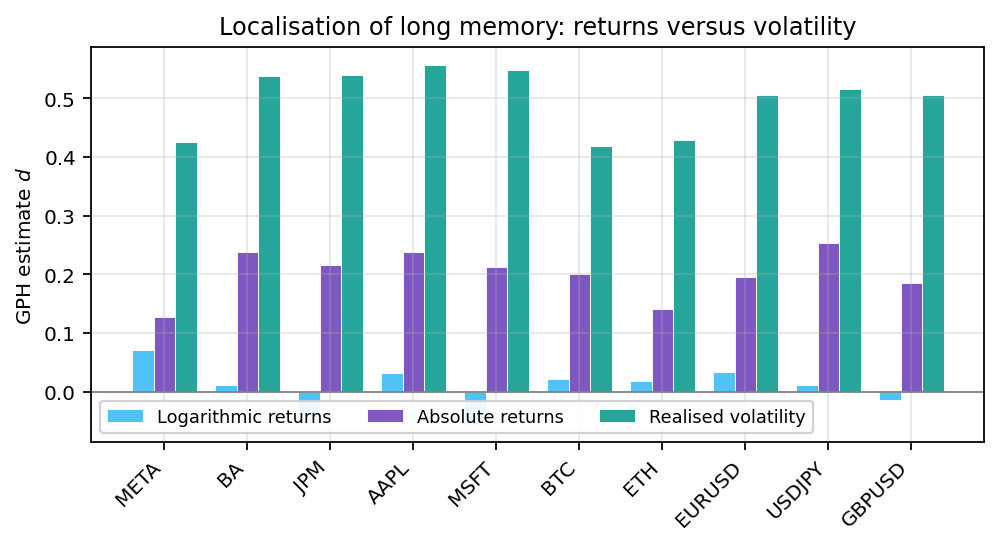
\includegraphics[width=\columnwidth]{fig_memory_localization_en.png}
\caption{Localisation of long memory. GPH estimates of the fractional integration parameter $d$ for
logarithmic returns, absolute returns and realised volatility, by asset.}
\label{fig:loc}
\end{figure}

The dispersion of the estimates is reported in Table~\ref{tab:mem}. It is substantial in relative
terms: the standard deviation of $\hat d(t)$ ranges from $0.052$ for ETH to $0.136$ for BA, and the
full range reaches half of the mean, with $\hat d$ varying between $0.329$ and $0.747$ for MSFT.
A parameter that fluctuates over an interval of that width within a single asset cannot plausibly
be treated as a constant of the data-generating process.

\begin{table}[t]
\centering
\caption{Local memory of realised volatility. Mean and standard deviation of the windowed estimate
over $W=500$ observations, the minimum value, the mean Hurst exponent, and the significance of the
structural break detected by the CUSUM test.}
\label{tab:mem}
\begin{tabular}{lccccc}
\toprule
\textbf{Asset} & $\bar{\hat d}$ & $\sigma(\hat d)$ & $\min \hat d$ & $\bar H$ & $p_{\mathrm{CUSUM}}$ \\
\midrule
META   & 0.426 & 0.094 & 0.295 & 0.897 & $<0.001$ \\
BA     & 0.538 & 0.136 & 0.354 & 0.937 & $<0.001$ \\
JPM    & 0.539 & 0.122 & 0.332 & 0.911 & $<0.001$ \\
AAPL   & 0.556 & 0.104 & 0.359 & 0.951 & 0.003 \\
MSFT   & 0.548 & 0.115 & 0.329 & 0.948 & $<0.001$ \\
BTC    & 0.419 & 0.102 & 0.229 & 0.905 & 0.056 \\
ETH    & 0.430 & 0.052 & 0.281 & 0.912 & 0.448 \\
EURUSD & 0.506 & 0.102 & 0.292 & 0.932 & $<0.001$ \\
USDJPY & 0.516 & 0.124 & 0.240 & 0.915 & $<0.001$ \\
GBPUSD & 0.505 & 0.077 & 0.265 & 0.939 & 0.061 \\
\bottomrule
\end{tabular}
\end{table}

\subsection{The strength of memory is non-stationary and collapses in crises}

The local estimates are far from constant, and the formal tests confirm what the trajectories
display. The CUSUM test detects a structural shift in $\hat d(t)$ for seven of the ten assets at the
5\,\% level, with $p$-values below $0.005$ in five cases and below $0.001$ in four; the
difference between the mean local memory in crisis and in calm windows is significant for the
same seven assets. The direction is consistent in every significant case: the memory is weaker in
crisis. Aggregated over the ten assets, the mean local estimate falls from $0.52$ in calm periods
to $0.45$ in crisis periods, a decrease of approximately $13\%$.

Figure~\ref{fig:crisis} contrasts the regime means asset by asset, with the exact values
and the significance of each regime difference reported in Table~\ref{tab:breaks}, and
Fig.~\ref{fig:mem} shows the corresponding trajectories. The most pronounced collapse occurs during
the 2022 interest-rate tightening cycle, when the local memory of equities and currency pairs
falls synchronously from the $0.65$--$0.75$ range to $0.30$--$0.45$: the memory of volatility
"collapses" against the background of the crisis, the long-range dependencies lose strength and
the process moves closer to short memory. This effect is qualitatively consistent with the
observations reported in the literature for crisis periods \cite{vogl2023hurst,choi2025three}.

\begin{figure}[t]
\centering
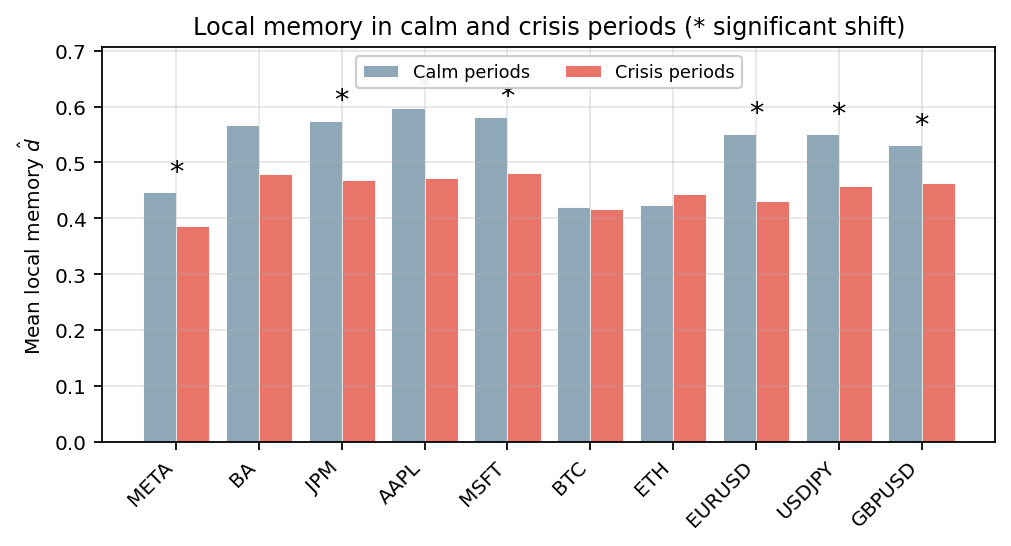
\includegraphics[width=\columnwidth]{fig_crisis_en.png}
\caption{Mean local memory in calm and in crisis periods. An asterisk marks a significant difference
between the two regimes (Welch $t$-test).}
\label{fig:crisis}
\end{figure}

\begin{figure}[t]
\centering
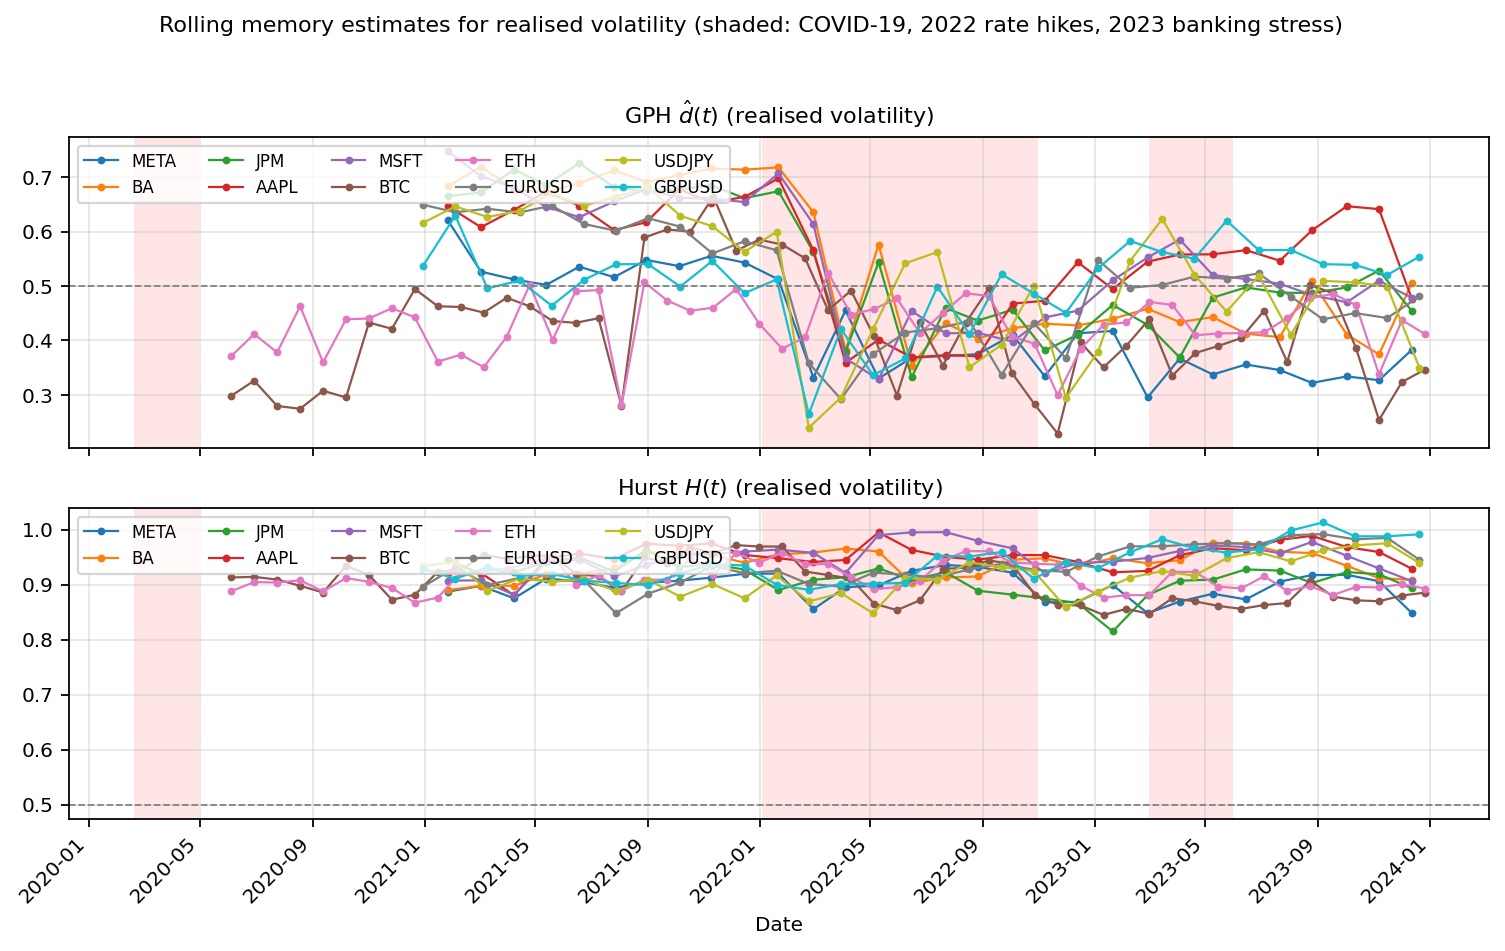
\includegraphics[width=\columnwidth]{paper_memory_en.png}
\caption{Rolling estimates $\hat d(t)$ and $H(t)$ for realised volatility; crisis periods are
highlighted.}
\label{fig:mem}
\end{figure}

Cryptocurrencies constitute the notable exception. For BTC and ETH neither the CUSUM test nor the
regime comparison rejects the null ($p_{\mathrm{CUSUM}}=0.056$ and $0.448$;
$p_{\mathrm{Welch}}=0.906$ and $0.159$), and the crisis and calm means coincide to within
$0.004$ and $0.019$ respectively. This pattern is consistent with the distinctive regime dynamics
of crypto markets, which exhibit a persistent high-frequency component and are less sensitive to
the monetary-policy channel, and it warrants separate study.

\begin{table}[t]
\centering
\caption{Structural breaks in the local memory estimate and the comparison of memory regimes.
$p_{\mathrm{CUSUM}}$ refers to the structural-break test on the trajectory of $\hat d(t)$;
$p_{\mathrm{Welch}}$ to the comparison of the mean local memory in crisis and calm windows.}
\label{tab:breaks}
\begin{tabular}{lcccc}
\toprule
\textbf{Asset} & $p_{\mathrm{CUSUM}}$ & $\bar{\hat d}_{\mathrm{crisis}}$ &
$\bar{\hat d}_{\mathrm{calm}}$ & $p_{\mathrm{Welch}}$ \\
\midrule
META   & $<0.001$ & 0.386 & 0.446 & 0.050 \\
BA     & $<0.001$ & 0.480 & 0.568 & 0.088 \\
JPM    & $<0.001$ & 0.469 & 0.574 & 0.021 \\
AAPL   & 0.003   & 0.472 & 0.598 & 0.008 \\
MSFT   & $<0.001$ & 0.480 & 0.582 & 0.037 \\
BTC    & 0.056   & 0.416 & 0.420 & 0.906 \\
ETH    & 0.448   & 0.443 & 0.424 & 0.159 \\
EURUSD & $<0.001$ & 0.430 & 0.551 & 0.001 \\
USDJPY & $<0.001$ & 0.458 & 0.550 & 0.046 \\
GBPUSD & 0.061   & 0.463 & 0.531 & 0.050 \\
\bottomrule
\end{tabular}
\end{table}

\subsection{The local memory estimate improves volatility forecasts}

Adding the local memory features $\hat d_t$ and $\Delta\hat d_t$ to HAR-RV improves the
out-of-sample forecast for all ten assets in terms of MSE, with an average gain of $+7.1\%$, and
for eight of the ten assets in terms of QLIKE, with an average gain of $+1.8\%$. The gains are
concentrated in the volatile instruments: $+26.9\%$ for META and $+16.1\%$ for BTC, and reach
$+8.5\%$ and $+6.4\%$ for EURUSD and USDJPY. The two assets for which the QLIKE gain is negative
(MSFT, $-5.7\%$; GBPUSD, $-0.3\%$) nevertheless exhibit positive MSE gains, which indicates that
the memory features improve the point forecast while occasionally shifting the estimated
conditional distribution towards the tails. Fig.~\ref{fig:har} displays the gains asset by asset, and Table~\ref{tab:har}
reports the underlying loss levels.

\begin{figure}[t]
\centering
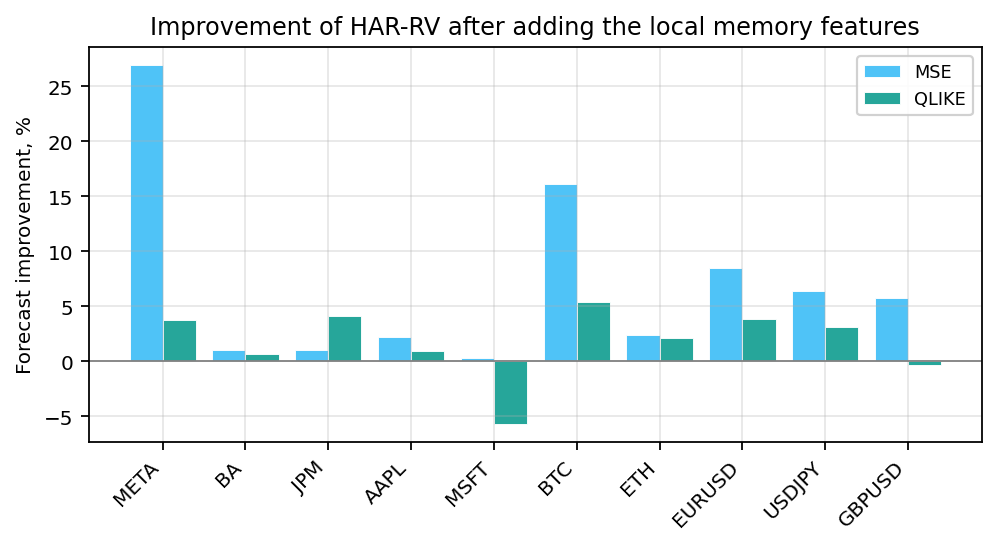
\includegraphics[width=\columnwidth]{fig_har_improvement_en.png}
\caption{Improvement of the HAR-RV forecast after adding the local memory features $\hat d_t$ and
$\Delta\hat d_t$, in per cent, by asset and by loss function.}
\label{fig:har}
\end{figure}

\begin{table}[t]
\centering
\caption{HAR-RV and its memory-augmented extension. $\Delta$MSE and $\Delta$QLIKE are the
percentage improvements in mean squared error and in QLIKE loss obtained by adding $\hat d_t$ and
$\Delta\hat d_t$ to the regressor set.}
\label{tab:har}
\begin{tabular}{lcccc}
\toprule
\textbf{Asset} & $\mathrm{QLIKE}_{\mathrm{base}}$ & $\mathrm{QLIKE}_{\mathrm{ext}}$ &
$\Delta$MSE (\%) & $\Delta$QLIKE (\%) \\
\midrule
META   & 0.01222 & 0.01176 & $+26.9$ & $+3.8$ \\
BA     & 0.00402 & 0.00399 & $+1.0$  & $+0.6$ \\
JPM    & 0.00348 & 0.00334 & $+1.0$  & $+4.1$ \\
AAPL   & 0.00449 & 0.00445 & $+2.2$  & $+0.9$ \\
MSFT   & 0.00426 & 0.00451 & $+0.3$  & $-5.7$ \\
BTC    & 0.00832 & 0.00787 & $+16.1$ & $+5.4$ \\
ETH    & 0.01254 & 0.01228 & $+2.4$  & $+2.1$ \\
EURUSD & 0.00360 & 0.00346 & $+8.5$  & $+3.8$ \\
USDJPY & 0.00827 & 0.00802 & $+6.4$  & $+3.1$ \\
GBPUSD & 0.00703 & 0.00705 & $+5.8$  & $-0.3$ \\
\bottomrule
\end{tabular}
\end{table}

This result is of principle importance in two respects. First, it shows that non-stationary memory
carries predictable information: the local estimate is not an artefact of the estimation procedure
but a genuine property of the data that is stable enough to improve a benchmark forecast out of
sample. Second, it directly motivates the construction of Section~\ref{sec:memadapt}: if a simple
linear regressor $\hat d_t$ improves the forecast, then an architecture that regulates its whole
attention scheme by the local strength of the memory has the potential to deliver a larger gain.

\subsection{Static attention mechanisms degrade differently across memory regimes}

All three attention mechanisms degrade when the memory regime switches from low to high, but they
do so to very different degrees, as reported in Table~\ref{tab:attn} and illustrated in
Fig.~\ref{fig:attn}. Full self-attention loses $+51\%$ in RMSE, the two-path MultiFeature
mechanism $+50\%$, and the sparse ProbSparse mechanism $+143\%$.

\begin{figure}[t]
\centering
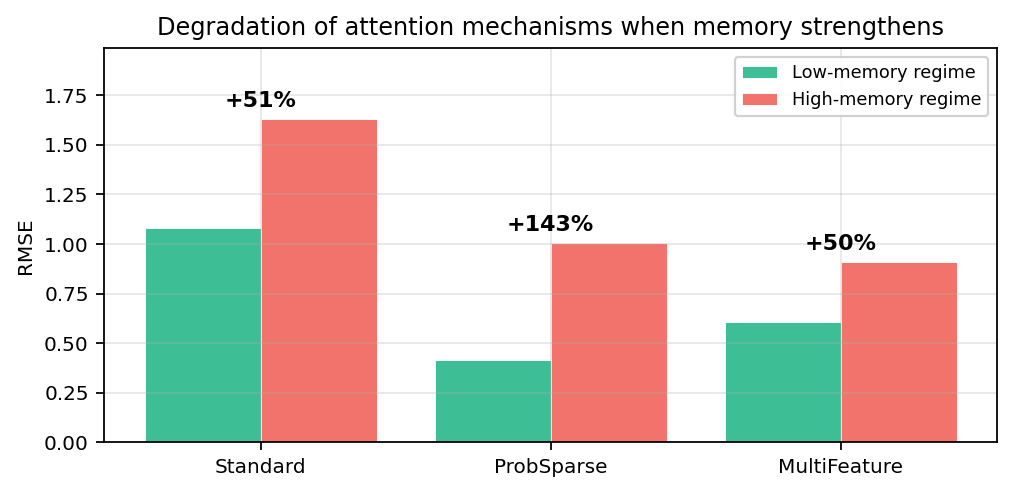
\includegraphics[width=\columnwidth]{fig_attention_deg_en.png}
\caption{Degradation of the attention mechanisms across memory regimes: RMSE in the low-memory and
in the high-memory regime, with the relative growth indicated.}
\label{fig:attn}
\end{figure}

\begin{table}[t]
\centering
\caption{Quality of the attention mechanisms by memory regime, evaluated on the same test sample.
The last two columns give the relative RMSE growth from the low-memory to the high-memory regime
and the $R^2$ on the full sample.}
\label{tab:attn}
\setlength{\tabcolsep}{3.4pt}
\begin{tabular}{lccccc}
\toprule
\textbf{Mechanism} & \textbf{RMSE low} & \textbf{RMSE high} & \textbf{Growth, \%} &
\textbf{$R^2$} & \textbf{Theil $U^2$} \\
\midrule
Standard     & 1.078 & 1.628 & $+51$  & 0.984 & 4.036 \\
ProbSparse   & 0.415 & 1.006 & $+143$ & 0.995 & 2.171 \\
MultiFeature & 0.608 & 0.911 & $+50$  & 0.994 & 2.369 \\
\bottomrule
\end{tabular}
\end{table}

Three conclusions follow. First, \emph{every static mechanism degrades when the memory is
strong}: the error rises for all three, which is direct empirical confirmation that a fixed
attention scheme is inconsistent with the structure of the data when long-range dependencies
intensify. Second, \emph{the sparse mechanism degrades most sharply}: ProbSparse is the best
mechanism in the low-memory regime (RMSE $=0.415$), yet it loses more than half its accuracy when
memory strengthens, because a top-$k$ selection with a fixed budget discards exactly the
informative long links. This is a concrete demonstration of the limitation of sparsity under
non-stationary memory. Third, \emph{the two-path architecture is the most robust}: MultiFeature
achieves the smallest absolute error in the high-memory regime (RMSE $=0.911$), and its variate
path, which processes interactions between features, partially compensates for the loss of long
temporal context in the temporal path. This suggests that the decomposition of the representation
across scales --- the idea underlying both HAR and the adaptive design of
Section~\ref{sec:memadapt} --- is more consequential for long-memory series than the raw
sparsity of the attention map.

The joint conclusion is quantitative rather than rhetorical: no static attention mechanism is
optimal in both regimes, and the quality of a mechanism depends systematically on the current
strength of the long-term memory. A mechanism that adapts its scheme to the local memory is
therefore potentially able to dominate every fixed alternative.

\section{Discussion}\label{sec:discussion}

\subsection{Interpretation}

Taken together, the four experiments support a single conclusion: the long-term memory of
volatility is not a static property of the series but a dynamic one, and this dynamics carries
usable information. Three implications follow for the modelling of volatility.

First, the classical econometric models are mis-specified in a specific and measurable way. The
damage is not diffuse but concentrated: the fixed memory structure produces its largest errors
exactly at regime changes, which are the periods in which risk measurement matters most.

Second, the transformer reading of attention as a learnable autocorrelation function is
substantive rather than metaphorical, and it carries a design consequence. An attention scheme
that does not depend on the estimated memory cannot be optimal across regimes, and this is
confirmed quantitatively: the degradation is not uniform across mechanisms but depends precisely
on how each mechanism treats long-range links.

Third, the predictive content of the local memory estimate is economically meaningful. A $7.1\%$
average reduction in the mean squared error of a benchmark model, obtained by adding two
regressors and no change to the model itself, is not a marginal improvement.

\subsection{Limitations and the critique of long-memory diagnostics}\label{sec:limitations}

The results must be interpreted in the light of the critique developed by Gatheral, Jaisson and
Rosenbaum \cite{gatheral2018rough}. Their analysis shows that the log-volatility of equity indices
behaves essentially as a fractional Brownian motion with $H$ of order $0.1$, and that classical
long-memory diagnostics --- the scaling behaviour of the integrated variance, the behaviour of
fractionally differentiated series --- then produce a spurious long-memory conclusion. If a
comparable mechanism operates in realised volatility, the interpretation of $\hat d$ as a
structural parameter of the data-generating process is not warranted, and the estimates reported
here should be read as \emph{local diagnostics of persistence} rather than as estimates of a true
fractional integration parameter. The paper's contribution has been framed accordingly: the
object of study is the \emph{time variation} of the local estimate, not the asymptotic behaviour of
the autocovariance function.

This limitation does not invalidate the present findings, but it changes their interpretation, and
we prefer to state this explicitly. A quantity that is not a structural parameter of the process
may still be informative about the state of the market, in the same way that a moving average of
volatility is informative about the level of volatility without being a parameter of any model.
The gains in forecast accuracy reported in Section~\ref{sec:results} are estimated out of sample
against a fixed benchmark under an expanding window, and are therefore not explained by the mere
presence of a persistent regressor. Moreover, the direction of the regime effect --- memory
weakening in crises --- is consistent with the existing literature on crisis dynamics of the Hurst
exponent \cite{vogl2023hurst,choi2025three}, which was obtained without the use of the
diagnostics we employ.

A second qualification concerns the interpretation of the mechanism-level results. The pilot
experiment on attention mechanisms is deliberately small: three mechanisms, one feature set, one
asset sample and a single crisis episode. It is designed to establish that the interaction
between the attention scheme and the memory regime is real and is not uniform across mechanisms,
and it succeeds in that purpose; it is not designed to provide precise estimates of the magnitude
of the effect, which will require the full comparison programme of Section~\ref{sec:outlook}.

\subsection{Threats to validity}

Three threats to the internal and external validity of the conclusions should be recorded.

\emph{Window specification.} The trajectories $\hat d(t)$ depend on the width $W$ of the rolling
window. A narrower window increases the temporal resolution but inflates the sampling variance
of the estimate, which would tend to exaggerate the apparent non-stationarity; a wider window
smooths the trajectories and would tend to understate it. The finding of a regime effect is
therefore conservative with respect to this trade-off, and the reported effect sizes should be
read as lower bounds on the true dispersion of the memory.

\emph{Regime assignment.} Crisis windows are assigned ex ante from the calendar. An alternative
would be to identify regimes endogenously, from the estimated memory trajectory itself, but this
would introduce a circularity between the object of study and the classification of the data.
Bootstrap confidence intervals for the regime differences provide a partial safeguard against
the arbitrariness of the crisis labels.

\emph{Sample size.} The sample covers a single five-year window containing the COVID-19 shock but
not a longer sequence of independent crises. The regime statistics are therefore based on a
moderate number of events, and the inference for the crypto subsample, where no significant
difference is detected, must be correspondingly conservative: the absence of a significant
difference for BTC and ETH is not evidence of the absence of regime dependence, but it does
establish that the regime effect observed for the other eight assets is not universal.

\subsection{Towards Memory-Adaptive Attention}\label{sec:outlook}

The programme that follows from the present results has three components. The first is a
mathematical formalisation of the adaptive mechanism of \eqref{eq:memad}: the relation between the
structure of attention and the autocovariance function of fractionally integrated processes, the
appropriate temperature schedule, and the truncation rule for the effective horizon. The second is
the implementation of a differentiable local memory estimator embedded in the architecture, with
the regularisation towards the classical estimators discussed above. The third is the extension
of the evaluation to a full comparison with econometric and neural baselines --- HAR-RV, FIGARCH
and ARFIMA on the econometric side, LSTM, Informer, PatchTST and DLinear on the neural side ---
culminating in the construction and backtesting of VaR and ES estimates on the basis of the
improved forecasts, with the unconditional and conditional coverage tests as the criterion.

\section{Conclusion}\label{sec:concl}

The paper has investigated the non-stationarity of long-term memory in the volatility of financial
time series, its predictive value, and the consequences of this phenomenon for the design of
attention mechanisms. The empirical evidence, obtained on a sample of ten assets from three asset
classes over 2019--2023, is unambiguous on three points. Long-term memory in volatility is
strong and is clearly stronger than in returns, with $\hat d$ of the order of $0.42$--$0.56$
against values indistinguishable from zero for logarithmic returns. The strength of this memory is
significantly non-stationary for seven of the ten assets and weakens systematically in crisis
periods, the mean local estimate falling from $0.52$ to $0.45$. And the local memory estimate
carries independent forecasting information, improving HAR-RV by $+7.1\%$ in MSE on average and by
$+1.8\%$ in QLIKE for eight of the ten assets.

These results carry a direct methodological consequence. Because the self-attention mechanism is a
learnable autocorrelation function, and because the attention schemes currently used in the
state-of-the-art long-horizon architectures are specified a priori, no static scheme can be
optimal across memory regimes; the quantitative degradation reported here --- from $+50\%$ for the
most robust mechanism to $+143\%$ for the sparsest --- measures the size of the gap that an
adaptive mechanism would have to close. The Memory-Adaptive Attention construction proposed
above, in which a differentiable local memory estimator controls the effective context length and
the sparsity of attention, together with the recent results on the differentiable estimation of
Hurst and fractional integration parameters, provides a technically feasible route to closing it.

Finally, the present evidence should be read with the caveat stated in
Section~\ref{sec:limitations}: what has been demonstrated is that a local diagnostic of
persistence varies over time, that this variation is regime-linked, and that it is informative for
forecasting. Whether the underlying process is genuinely fractionally integrated, as opposed to
being rough with regime-dependent scaling, is a question that the recent literature has reopened
and that our estimates do not settle --- and that the subsequent chapters of the thesis are
addressing.

\section*{Acknowledgment}

The author thanks the Department of Probability Theory and Mathematical Statistics of the
Belarusian State University for the computational resources and for the discussion of the
results.

\begin{thebibliography}{99}

\bibitem{ding1993long}
D.~Z.~Ding, C.~W.~J.~Granger, and R.~F.~Engle, ``A long memory property of stock market prices
and a new model,'' \textit{J. Empirical Finance}, vol.~1, no.~1, pp.~1--28, 1993.

\bibitem{andersen2003modeling}
T.~G.~Andersen, T.~Bollerslev, F.~X.~Diebold, and P.~Labys, ``Modeling and forecasting
realized volatility,'' \textit{Econometrica}, vol.~71, no.~2, pp.~579--625, 2003.

\bibitem{baillie1996fractionally}
R.~T.~Baillie, T.~Bollerslev, and H.~O.~Mikkelsen, ``Fractionally integrated generalized
autoregressive conditional heteroskedasticity,'' \textit{J. Econometrics}, vol.~74, no.~1,
pp.~3--30, 1996.

\bibitem{banerjee2005modelling}
A.~Banerjee and G.~Urga, ``Modelling structural breaks, long memory and stock market
volatility: an overview,'' \textit{J. Econometrics}, vol.~129, no.~1--2, pp.~1--34, 2005.

\bibitem{beran1994statistics}
J.~Beran, \textit{Statistics for Long-Memory Processes}. London, U.K.: Chapman \& Hall/CRC, 1994.

\bibitem{bennedsen2022decoupling}
M.~Bennedsen, A.~Lunde, and M.~S.~Pakkanen, ``Decoupling the short- and long-term behavior of
stochastic volatility,'' \textit{J. Financial Econometrics}, vol.~20, no.~5, pp.~961--1006, 2022.

\bibitem{boros2024deep}
D.~Boros, et al., ``Deep learning the Hurst parameter of linear fractional processes and
assessing its reliability,'' arXiv:2401.01789, 2024.

\bibitem{choi2010long}
K.~Choi, W.-C.~Yu, and E.~Zivot, ``Long memory versus structural breaks in modeling and
forecasting realized volatility,'' \textit{J. International Money and Finance}, vol.~29, no.~5,
pp.~857--875, 2010.

\bibitem{choi2025three}
J.~Choi, ``The three-dimensional decomposition of volatility memory: level, tempo, and shape,''
arXiv:2512.02166, 2025.

\bibitem{christoffersen1998evaluating}
P.~F.~Christoffersen, ``Evaluating interval forecasts,'' \textit{International Economic Review},
vol.~39, no.~4, pp.~841--862, 1998.

\bibitem{corsi2009simple}
F.~Corsi, ``A simple approximate long-memory model of realized volatility,'' \textit{J. Financial
Econometrics}, vol.~7, no.~2, pp.~174--196, 2009.

\bibitem{csanady2024parameter}
B.~Csan\'ady, et al., ``Parameter estimation of long memory stochastic processes with deep neural
networks,'' arXiv:2410.03776, 2024.

\bibitem{chen2024cats}
S.~Chen, et al., ``Are self-attentions effective for time series forecasting?'' arXiv:2405.16877,
2024.

\bibitem{dipersio2024deep}
L.~Di~Persio and M.~Russo, ``Deep neural network model for Hurst exponent: learning from R/S
analysis,'' \textit{Mathematics}, vol.~12, no.~22, art.~3483, 2024.

\bibitem{gatheral2018rough}
J.~Gatheral, T.~Jaisson, and M.~Rosenbaum, ``Volatility is rough,'' \textit{Quantitative
Finance}, vol.~18, no.~6, pp.~933--949, 2018.

\bibitem{geweke1983estimation}
J.~Geweke and S.~Porter-Hudak, ``The estimation and application of long memory time series
models,'' \textit{J. Time Series Analysis}, vol.~4, no.~4, pp.~221--238, 1983.

\bibitem{granger1980long}
C.~W.~J.~Granger and R.~Joyeux, ``An introduction to long-memory time series models and
fractional differencing,'' \textit{J. Time Series Analysis}, vol.~1, no.~1, pp.~15--29, 1980.

\bibitem{hosking1981fractional}
J.~R.~M.~Hosking, ``Fractional differencing,'' \textit{Biometrika}, vol.~68, no.~1, pp.~165--176,
1981.

\bibitem{hurst1951long}
H.~E.~Hurst, ``Long-term storage capacity of reservoirs,'' \textit{Transactions of the American
Society of Civil Engineers}, vol.~116, no.~1, pp.~770--799, 1951.

\bibitem{kupiec1995techniques}
P.~H.~Kupiec, ``Techniques for verifying the accuracy of risk measurement models,''
\textit{J. Derivatives}, vol.~3, no.~2, pp.~73--84, 1995.

\bibitem{liu2024arma}
Y.~Liu, et al., ``Autoregressive moving-average attention mechanism for time series
forecasting,'' arXiv:2410.03159, 2024.

\bibitem{lo1991long}
A.~W.~Lo, ``Long-term memory in stock market prices,'' \textit{Econometrica}, vol.~59, no.~5,
pp.~1279--1313, 1991.

\bibitem{ma2023dbaformer}
M.~Ma, et al., ``DBAFormer: a double-branch attention transformer for long-term time series
forecasting,'' \textit{Human-Centric Intelligent Systems}, vol.~3, pp.~1--15, 2023.

\bibitem{makarava2025differentiable}
N.~Makarava, et al., ``Differentiable neural network layer for estimating Hurst and anomalous
diffusion exponents,'' \textit{J. Physics A: Mathematical and Theoretical}, vol.~58, art.~265002,
2025.

\bibitem{mandelbrot1968fractional}
B.~B.~Mandelbrot and J.~W.~Van~Ness, ``Fractional Brownian motions, fractional noises and
applications,'' \textit{SIAM Review}, vol.~10, no.~4, pp.~422--437, 1968.

\bibitem{mikosch2004non}
T.~Mikosch and C.~Starica, ``Non-stationarities in financial time series, the long-range
dependence, and the IGARCH effects,'' \textit{Review of Economics and Statistics}, vol.~86,
no.~1, pp.~378--390, 2004.

\bibitem{nie2023time}
Y.~Nie, et al., ``A time series is worth 64 words: long-term forecasting with transformers,''
in \textit{Proc. Int. Conf. Learning Representations (ICLR)}, 2023.

\bibitem{palma2007long}
W.~Palma, \textit{Long-Memory Time Series: Theory and Methods}. Hoboken, NJ, USA: Wiley, 2007.

\bibitem{patton2011volatility}
A.~J.~Patton, ``Volatility forecast comparison using imperfect volatility proxies,''
\textit{J. Econometrics}, vol.~160, no.~1, pp.~246--256, 2011.

\bibitem{philipper2024adaptive}
C.~Philipper, et al., ``An adaptive temporal attention mechanism to address distribution shifts,''
in \textit{ICLR Workshop on Agents and Tools for Multi-Task Learning}, 2024.

\bibitem{pipiras2017long}
V.~Pipiras and M.~S.~Taqqu, \textit{Long-Range Dependence and Self-Similarity}. Cambridge, U.K.:
Cambridge Univ.\ Press, 2017.

\bibitem{tay2022efficient}
Y.~Tay, et al., ``Efficient transformers: a survey,'' \textit{ACM Computing Surveys}, vol.~55,
no.~6, pp.~1--28, 2022.

\bibitem{teverovsky1999stock}
V.~Teverovsky, M.~S.~Taqqu, and W.~Willinger, ``A critical look at Lo's modified R/S
statistic,'' \textit{J. Statistical Planning and Inference}, vol.~80, no.~1--2, pp.~211--227, 1999.

\bibitem{vaswani2017attention}
A.~Vaswani, et al., ``Attention is all you need,'' in \textit{Advances in Neural Information
Processing Systems}, vol.~30, pp.~5998--6008, 2017.

\bibitem{vogl2023hurst}
M.~Vogl, ``Hurst exponent dynamics of S\&P 500 returns: implications for market efficiency,
long memory, multifractality and financial crises predictability,'' \textit{Chaos, Solitons \&
Fractals}, vol.~166, art.~112884, 2023.

\bibitem{wen2023transformers}
Q.~Wen, et al., ``Transformers in time series: a survey,'' in \textit{Proc. Int. Joint Conf.
Artificial Intelligence (IJCAI)}, pp.~4584--4592, 2023.

\bibitem{wu2021autoformer}
H.~Wu, et al., ``Autoformer: decomposition transformers with auto-correlation for long-term series
forecasting,'' in \textit{Advances in Neural Information Processing Systems}, vol.~34,
pp.~22419--22430, 2021.

\bibitem{zhang2025twilight}
Z.~Zhang, et al., ``Twilight: adaptive attention sparsity with hierarchical top-p pruning,''
arXiv:2502.02770, 2025.

\bibitem{zhou2021informer}
H.~Zhou, et al., ``Informer: beyond efficient transformer for long sequence time-series
forecasting,'' in \textit{Proc. AAAI Conf. Artificial Intelligence}, vol.~35, no.~12,
pp.~11106--11115, 2021.

\bibitem{zhou2022fedformer}
T.~Zhou, et al., ``FEDformer: frequency enhanced decomposed transformer for long-term series
forecasting,'' in \textit{Proc. Int. Conf. Machine Learning}, PMLR, pp.~27268--27286, 2022.

\bibitem{zhou2024sdformer}
Z.~Zhou, ``SDformer: transformer with spectral filter and dynamic attention for multivariate time
series long-term forecasting,'' in \textit{Proc. Thirty-Third Int. Joint Conf. Artificial
Intelligence (IJCAI)}, pp.~5689--5697, 2024.

\bibitem{cherenda2020research}
S.~N.~Cherenda, et al., \textit{English: Communication in Science Community}. Minsk, Belarus:
Belarusian State University, 2020.

\end{thebibliography}

\end{document}
